\section{Lec 21}
The Einstein tensor expressed with the components of $h_{\mu \nu }$ becomes
\begin{align}
	G_{00} &= 2 \nabla ^{2}\Psi + \partial_{k}\partial_{l}s^{kl} \label{eq:psi}\\
	G_{0j} &= -\frac{1}{2} \nabla ^{2}w_{j}+\frac{1}{2}\partial_{j}\partial_{k}w^{k} + 2 \partial_{0}\partial_{j}\Psi + \partial_{0}\partial_{k}s^{k}_{j} \\
	G_{ij} &= \left( \delta _{ij} \nabla ^{2} - \partial_{i}\partial_{j} \right)\left( \phi -\Psi  \right) + \delta _{ij}\partial_{0}\partial_{k}w^{k} - \partial_{0}\partial_{( i}w_{j)} \nonumber \\
	       & +2\delta _{ij}\partial_{0}^{2}\Psi - \Box s_{ij} + 2\partial_{k}\partial_{( i}s_{j)}^{k}-\delta _{ij}\partial_{k}\partial_{l}s^{kl} 
\end{align}
Let's remember, the Einstein Equations are
\[
G_{\mu \nu } = R_{\mu \nu } -\frac{1}{2}g_{\mu \nu }R = 8\pi G T_{\mu \nu }
\]
When you try to solve this equation here, instead of the full Ricci tensor it's ok to use the linearized expression found yesterday, to put the minkowsky metric instead of $g_{\mu \nu }$ since otherwise we would have second order in $h$ in that factor because the Ricci scalar is already first order in \emph{h}. On the right-hand side $8\pi G$ is zero-th order in \emph{h} and $T_{\mu \nu } $ is linear in \emph{h}\par
\[
G_{\mu \nu } = R_{\mu \nu } -\eta _{\mu \nu }R = 8\pi G T_{\mu \nu }
\]
If we know $T_{00 }$\footnote{energy density, via the sources} and $s_{ij}$, We can find $\Psi $ from eq.\ref{eq:psi} and
\[
G_{00} = 8\pi G T_{00}
\]
also, since there is no time derivative, $\Psi $ does not propagate.\par
The $G_{0i}$ term specifies $w_{j}$ in terms of $\Psi, s_{ij}, T_{0i}$. The $G_{ij}$ term specifies $\phi$. Always without a time derivative. \par
So as probably just said the propagating terms are all in the $s_{ij}$ component of the metric.\par
\subsubsection{Gauge transformations of components of $h_{\mu \nu }$}

We already discussed the family of gauge transformations made from
\[
h_{\mu \nu } = h_{\mu \nu } + \partial_{\mu }\xi _{\nu }+\partial_{\nu }\xi _{\mu }
\]
What does it look like plugged in
\begin{itemize}
\item $h_{00} = -2\phi $
\item $h_{0i} = w_{i}$
\item $h_{ij} = 2s_{ij} -2\Psi \delta _{ij}$ 
\end{itemize}
Let's start from $h_{00} = -2\phi $
\begin{gather*}
h_{00} \to  h_{00}+\partial_{0}\xi _{0}+\partial_{0}\xi_{0} = h_{00} +2\partial_{0}\xi _{0} = h_{00} -2\partial_{0}\xi ^{0}\\
\to -2\phi  = -2\phi - 2\partial_{0}\xi ^{0} \to  \phi = \phi +\partial_{0}\xi ^{0}
\end{gather*}
About $h_{0i} = w_{i} = w^{i}$:
\begin{gather*}
h_{0i} \to  h_{0i} + \partial_{0}\xi _{i} + \partial_{i}\xi _{0} \to w_{i} = w_{i} +\partial_{0}\xi^{i} -\partial_{i}\xi^{0}
\end{gather*}
Lastly, about $h_{ij} = 2s_{ij}-2\Psi \delta _{ij}$, we will split in the two components
\begin{gather*}
\Psi  = -\frac{1}{6}\delta _{ij}h_{ij} \\
\Psi \to -\frac{1}{6} \delta _{ij}\left( h_{ij}+\partial_{i}\xi ^{j}+\partial_{j}\xi ^{i} \right) = \Psi -\frac{1}{3}\partial_{i}\xi ^{i}
\end{gather*}
last step we used the delta to make \emph{j} to \emph{i}. While for $s_{ij}$
\begin{gather*}
	2s_{ij} = h_{ij} +2\Psi \delta _{ij}  \to  s_{ij} = \frac{h_{ij}}{2} + \Psi \delta _{ij}\\
	s_{ij} \to \frac{h_{ij} +\partial_{i}\xi ^{j}+\partial_{j}\xi ^{i}}{2} + \delta _{ij}\left( \Psi - \frac{1}{3}\partial_{k}\xi ^{k} \right) \\
	s_{ij} \to s_{ij} + \frac{\partial_{i}\xi ^{j}+\partial_{j}\xi ^{i}}{2} -\frac{1}{3}\partial_{k}\xi ^{k}\delta _{ij} 
\end{gather*}
Now, about degrees of freedom we see that
\begin{itemize}
\item $\phi  \to  1$, it's a scalar
\item $\Psi  \to  1$, same reason
\item $w_{i} \to  3$ it's a vector
\item $s_{ij}\to 5$, because it's symmetric but also traceless.	
\end{itemize}
We are ok. We foresaw 10 degrees of freedom and we got them. These will be used to simplify equations.

\subsubsection{Transverse Gauge}

The \textbf{transverse gauge} is a specific choice of gauge condition in linearized gravity that simplifies the equations by imposing constraints on the metric perturbations $h_{\mu \nu }$. 
We saw that the left hand side of the Einstein Equations can be written as function of $\phi ,\Psi ,w_{i},s_{ij}$. But they are a lot, what we can do with \emph{gauge freedom} is to choose a specific gauge that makes EEs easier. The \emph{transverse gauge }is defined by imposing this condition
\[
\partial_{i}s^{ij} = 0	
\]
while it's gauge transformations is 
\[
\partial_{i} s^{ij} \to \partial_{i}s^{ij} + \frac{\partial_{i}\partial_{j}\xi ^{i}+\partial_{j}\partial_{i}\xi ^{i}}{2} - \frac{\partial_{j}\partial_{k}\xi ^{k}}{3} = 0
\]
Since setting $\partial_{i}s^{ij}$ only involves $\xi ^{i}$ and not $\xi ^{0}$, we can use the latter to set
\[
\partial_{i}w^{i} = 0 
\]
and the gauge transformations is
\[
\partial_{i}w^{i} \to \partial_{i}w^{i}+ \partial_{0}\partial_{i}\xi ^{i} - \partial_{i}\partial_{i}\xi ^{0} = 0
\]
The transverse gauge is defined by imposing these conditions

\subsection{Deflection of light}
\bigskip
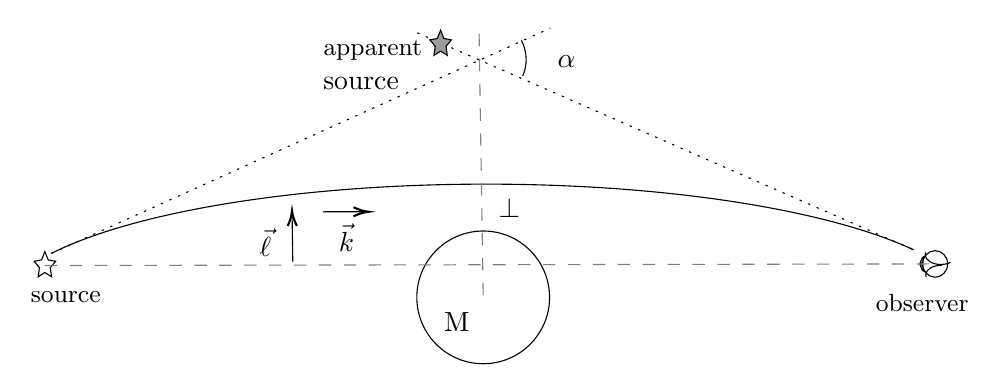
\begin{tikzpicture}[x=0.5pt,y=0.5pt,yscale=-1,xscale=1]\label{imm:deflight}
%uncomment if require: \path (0,300); %set diagram left start at 0, and has height of 300

%Shape: Circle [id:dp771951895826762]
\draw   (301.5,193.54) .. controls (301.5,167.05) and (322.97,145.57) .. (349.46,145.57) .. controls (375.95,145.57) and (397.43,167.05) .. (397.43,193.54) .. controls (397.43,220.03) and (375.95,241.5) .. (349.46,241.5) .. controls (322.97,241.5) and (301.5,220.03) .. (301.5,193.54) -- cycle ;
%Shape: Star [id:dp6359593737575958]
\draw   (32.7,160.5) -- (35.12,166.48) -- (40.51,167.44) -- (36.61,172.09) -- (37.53,178.66) -- (32.7,175.56) -- (27.88,178.66) -- (28.8,172.09) -- (24.9,167.44) -- (30.29,166.48) -- cycle ;
%Shape: Moon [id:dp9355776016007231]
\draw   (668.72,174.98) .. controls (667,174.98) and (665.61,172.47) .. (665.61,169.37) .. controls (665.61,166.27) and (667,163.76) .. (668.72,163.76) .. controls (667.7,164.8) and (667.01,166.92) .. (667.01,169.37) .. controls (667.01,171.82) and (667.7,173.95) .. (668.72,174.98) -- cycle ;
%Shape: Ellipse [id:dp9808296411167978]
\draw   (667.01,169.37) .. controls (667.01,164.07) and (671.06,159.78) .. (676.07,159.78) .. controls (681.07,159.78) and (685.13,164.07) .. (685.13,169.37) .. controls (685.13,174.67) and (681.07,178.96) .. (676.07,178.96) .. controls (671.06,178.96) and (667.01,174.67) .. (667.01,169.37) -- cycle ;
%Shape: Ellipse [id:dp5309857774037612]
\draw  [fill={rgb, 255:red, 0; green, 0; blue, 0 }  ,fill opacity=1 ] (665.17,169.37) .. controls (665.17,168.48) and (665.37,167.76) .. (665.61,167.76) .. controls (665.86,167.76) and (666.06,168.48) .. (666.06,169.37) .. controls (666.06,170.26) and (665.86,170.98) .. (665.61,170.98) .. controls (665.37,170.98) and (665.17,170.26) .. (665.17,169.37) -- cycle ;
%Shape: Arc [id:dp525233388687705]
\draw  [draw opacity=0] (687.2,168.33) .. controls (685.28,169.25) and (682.88,169.8) .. (680.28,169.8) .. controls (673.99,169.8) and (668.9,166.62) .. (668.9,162.69) .. controls (668.9,162.11) and (669.01,161.56) .. (669.21,161.02) -- (680.28,162.69) -- cycle ; \draw   (687.2,168.33) .. controls (685.28,169.25) and (682.88,169.8) .. (680.28,169.8) .. controls (673.99,169.8) and (668.9,166.62) .. (668.9,162.69) .. controls (668.9,162.11) and (669.01,161.56) .. (669.21,161.02) ;
%Shape: Arc [id:dp9530537025832931]
\draw  [draw opacity=0] (680.94,170.34) .. controls (680.85,170.33) and (680.76,170.33) .. (680.67,170.33) .. controls (674.39,170.33) and (669.3,173.41) .. (669.3,177.2) .. controls (669.3,177.78) and (669.41,178.33) .. (669.63,178.87) -- (680.67,177.2) -- cycle ; \draw   (680.94,170.34) .. controls (680.85,170.33) and (680.76,170.33) .. (680.67,170.33) .. controls (674.39,170.33) and (669.3,173.41) .. (669.3,177.2) .. controls (669.3,177.78) and (669.41,178.33) .. (669.63,178.87) ;
%Shape: Arc [id:dp5546436803794585]
\draw  [draw opacity=0] (37.19,161.87) .. controls (96.01,132.07) and (214.75,111.7) .. (351.64,111.7) .. controls (484.41,111.7) and (600.09,130.86) .. (660.61,159.2) -- (351.64,204.39) -- cycle ; \draw   (37.19,161.87) .. controls (96.01,132.07) and (214.75,111.7) .. (351.64,111.7) .. controls (484.41,111.7) and (600.09,130.86) .. (660.61,159.2) ;
%Straight Lines [id:da40594427389682397]
\draw  [dash pattern={on 0.84pt off 2.51pt}]  (37.19,161.87) -- (397.86,-0.97) ;
%Straight Lines [id:da8857728324479436]
\draw  [dash pattern={on 0.84pt off 2.51pt}]  (301.86,2.37) -- (660.61,159.2) ;
%Straight Lines [id:da47150359358950156]
\draw [color={rgb, 255:red, 128; green, 128; blue, 128 }  ,draw opacity=1 ] [dash pattern={on 4.5pt off 4.5pt}]  (346.52,3.03) -- (349.46,193.54) ;
%Straight Lines [id:da9767928107595374]
\draw [color={rgb, 255:red, 128; green, 128; blue, 128 }  ,draw opacity=1 ] [dash pattern={on 4.5pt off 4.5pt}]  (32.7,170.54) -- (676.07,169.37) ;
%Shape: Arc [id:dp8396531267879266]
\draw  [draw opacity=0] (378.05,33.5) .. controls (379.64,29.87) and (380.52,25.87) .. (380.52,21.67) .. controls (380.52,16.66) and (379.27,11.94) .. (377.06,7.78) -- (349.93,21.67) -- cycle ; \draw   (378.05,33.5) .. controls (379.64,29.87) and (380.52,25.87) .. (380.52,21.67) .. controls (380.52,16.66) and (379.27,11.94) .. (377.06,7.78) ;
%Shape: Star [id:dp875511273739857]
\draw  [fill={rgb, 255:red, 155; green, 155; blue, 155 }  ,fill opacity=1 ] (318.7,0.5) -- (321.12,6.48) -- (326.51,7.44) -- (322.61,12.09) -- (323.53,18.66) -- (318.7,15.56) -- (313.88,18.66) -- (314.8,12.09) -- (310.9,7.44) -- (316.29,6.48) -- cycle ;
%Straight Lines [id:da0849534276319821]
\draw    (211.86,167.7) -- (211.36,133) ;
\draw [shift={(211.33,131)}, rotate = 89.18] [color={rgb, 255:red, 0; green, 0; blue, 0 }  ][line width=0.75]    (10.93,-3.29) .. controls (6.95,-1.4) and (3.31,-0.3) .. (0,0) .. controls (3.31,0.3) and (6.95,1.4) .. (10.93,3.29)   ;
%Straight Lines [id:da4422372411664188]
\draw    (233.86,131.7) -- (264.67,131.67) ;
\draw [shift={(266.67,131.67)}, rotate = 179.94] [color={rgb, 255:red, 0; green, 0; blue, 0 }  ][line width=0.75]    (10.93,-3.29) .. controls (6.95,-1.4) and (3.31,-0.3) .. (0,0) .. controls (3.31,0.3) and (6.95,1.4) .. (10.93,3.29)   ;

% Text Node
\draw (319.33,202.67) node [anchor=north west][inner sep=0.75pt]   [align=left] {M};
% Text Node
\draw (358.67,120.33) node [anchor=north west][inner sep=0.75pt]   [align=left] { $\bot$};
% Text Node
\draw (20.67,187.67) node [anchor=north west][inner sep=0.75pt]   [align=left] {\small source};
% Text Node
\draw (631.33,189.67) node [anchor=north west][inner sep=0.75pt]   [align=left] {\small observer};
% Text Node
\draw (401.33,16.67) node [anchor=north west][inner sep=0.75pt]   [align=left] { $\alpha $};
% Text Node
\draw (232,6) node [anchor=north west][inner sep=0.75pt]   [align=left] {\small apparent\\source};
% Text Node
\draw (186,142.33) node [anchor=north west][inner sep=0.75pt]   [align=left] { $\vec{\ell}$};
% Text Node
\draw (243.33,138.67) node [anchor=north west][inner sep=0.75pt]   [align=left] { $\vec{k}$};
\end{tikzpicture} \par
\bigskip
Deflection of light, or \emph{gravitational lensing}, can be studied under two assumptions: static field, and transverse gauge (linearized gravity and weak field).\par
What we want is to write the Einstein Equations, because of transverse gauge and staticness (time derivative = 0), many terms are null.
\begin{align}
	G_{00}& = 2\nabla ^{2}\phi  + \partial_{k}\partial_{l}s^{kl} = 2\nabla ^{2}\phi \\
	G_{0j}& = -\frac{1}{2}\nabla ^{2}w_{j}+ \ldots +\ldots +\ldots  = -\frac{1}{2}\nabla ^{2}w_{j} \\
G_{ij} & = \left( \delta _{ij}\nabla ^{2}-\partial_{i}\partial_{j} \right)\left( \phi -\Psi  \right)- \Box s_{ij} 
\end{align}
Regarding $T_{\mu \nu }$, this is the source, and in our case, since the Sun (see fig. \ref{imm:deflight}) is at rest, we can take the NR form of it so
\[
T_{\mu \nu } = \begin{pmatrix}
\rho  & 0 & 0 & 0 \\
0 & 0 & 0 & 0 \\
0 & 0 & 0 & 0 \\
0 & 0 & 0 & 0
\end{pmatrix} 
\]
So we stay in the frame where the object that bends is at rest. With this \emph{energy-momentum tensor} 
\begin{align}
	G_{00} &= 2\nabla ^{2}\phi = 8\pi G \rho \\
	G_{0j} &= -\frac{1}{2}\nabla ^{2}w_{j} = 0 \\
	G_{ij} &= \left( \delta _{ij}\nabla ^{2}- \partial_{i}\partial_{j} \right)\left( \phi -\Psi  \right)- \nabla ^{2}s_{ij} = 0
\end{align}
note that the d'alembertian operator $\Box$ has become $\nabla ^{2}$ in the third equation, this because of staticness. That laplacian is in spatial coordinates.\footnote{ $\Box = \nabla ^{2} - \frac{1}{v^{2}}\partial_{t}^{2}$.}
Now we claim that, since $\nabla ^{2}w_{j} = 0$, if this condition has to be well-behaved at $\infty$, then the only solution is $w_{j} = 0$, in general the solution of $\frac{\partial^{2} }{\partial x^{2}} $ is $w = Ax+B$, in one dimension.\par
About the third equation, taking its trace, we get
\[
	\left(3\nabla ^{2} -\nabla ^{2}\right) \left( \phi -\Psi  \right) = 2\nabla ^{2}\left( \phi -\Psi  \right)= 0
\]
for the same reason, the solution is $\phi =\Psi  $. Plugging this solution in the full equation gets us $\nabla ^{2}s_{ij} = 0$, that, again, implies $s_{ij} = 0$ for a well-behaved solution.\par
The perturbed metric for static Newtonian sources, with staticness and transverse gauge is
\begin{equation}
ds^{2} = - \left( 1+2\phi  \right)dt^{2}+ \left( 1-2\phi  \right)\left( dx^{2}+dy^{2}+dz^{2} \right)
\end{equation}
and the perturbed metric is
\begin{equation}
h_{\mu \nu } = \begin{pmatrix}
-2\phi  & 0 & 0 & 0 \\
0 & -2\phi  & 0 & 0 \\
0 & 0 & -2\phi  & 0 \\
0 & 0 & 0 & -2\phi 
\end{pmatrix} 
\end{equation}
This is an improvement over the previous study on the motion of a slow particle, that allowed us to fill only the temporal part of the metric, while here, with a fast particle, we filled also the spatial section.\par
If I want to study the deflection of light, I have to study the trajectory of a photon. This can be written as 
\[
x^{\mu }\left( \lambda  \right) = x^{\mu }_{\left( 0 \right)}\left( \lambda  \right) + x^{\mu }_{\left( 1 \right)}\left( \lambda  \right)
\]
where we decomposed in two contributions:
\begin{itemize}
\item $x^{\mu }_{\left( 0 \right)}$ that solves the geodesic equation for a straight null path
\item $x^{\mu }_{\left( 1 \right)}$ that solves for the perturbation.
\end{itemize}
practically, these contribution are respectively of zero-th and first order in \emph{h}.
Consequentially, the four momentum can also be split into two contributions
\begin{gather*}
k^{\mu } = \frac{d x^{\mu }_{\left( 0 \right)}}{d \lambda } \\
\ell^{\mu } = \frac{d x^{\mu }_{\left( 1 \right)}}{d \lambda }
\end{gather*}
where we chose $\lambda $ in such a way that these are the four-momentum.\par
Let's look now at the geodesic equation
\[
\frac{d ^{2}x^{\mu }}{d \lambda ^{2} } + \Gamma ^{\mu }_{\alpha \beta } \frac{d x^{\alpha }}{d \lambda }\frac{d x^{\beta }}{d \lambda }
\]
In the linear regime, Christoffel connection is
\[
\Gamma ^{\mu }_{\alpha \beta } = \frac{1}{2}\eta ^{\mu \rho }\left[ \partial_{\alpha }h_{\rho \beta }+ \partial_{\beta }h_{\rho \alpha } - \partial_{\rho }h_{\alpha \beta } \right]
\]
and its only non-vanishing components are
\begin{gather*}
\Gamma ^{0}_{0i} = \Gamma ^{i}_{00} = \partial_{i}\phi  \\
\Gamma ^{i}_{jk} = \delta _{jk}\partial_{i}\phi - \delta _{ik}\partial_{j} \phi - \delta _{ij}\partial_{k}\phi  
\end{gather*}
The geodesic becomes
\begin{equation}
\frac{d }{d \lambda }\left( k^{\mu }+ \ell^{\mu } \right) + \Gamma ^{\mu }_{\alpha \beta }\left( k^{\alpha }+ \ell^{\alpha } \right)\left( k^{\beta }+\ell^{\beta } \right) = 0
\end{equation}
we can split this equation based on the orders
\begin{gather*}
\mathcal{O} \left( h^{0} \right)  \to  \frac{d k^{\mu }}{d \lambda }\\
\mathcal{O} \left( h^{2} \right) \to \frac{d \ell^{\mu }}{d \lambda } + \Gamma ^{\mu }_{\alpha \beta }k^{\alpha }k^{\beta } = 0
\end{gather*}

\paragraph{Geodesic Motion}
Be
\[
k^{\mu } = \left( \omega ,\vec{k} \right), k^{\mu }k_{\mu }=0, \omega = |\vec{k}|=k
\]
Let's see what happens with $\ell^{0}$:
\begin{gather*}
\frac{d \ell^{0}}{d \lambda } + \Gamma ^{0}_{0i}\omega k^{i} + \Gamma ^{0}_{i0}\omega k^{i} = 0 \\
\left( \Gamma ^{0}_{0i} = \Gamma ^{0}_{i0} = \partial_{i}\phi  \right) \\
\frac{d \ell^{0}}{d \lambda } + 2\partial_{i}\phi k^{i}k = 0 \\
\frac{d \ell^{0}}{d \lambda } = -2k\left( \vec{k}\cdot \vec{\nabla }\phi  \right)
\end{gather*}
while for the spatial part
\begin{equation}
	\frac{d \vec{\ell}}{d \lambda } = -2\left( k^{2}\nabla \phi - \vec{k}\left( \vec{k}\cdot \vec{\nabla }\phi  \right) \right) = -2k^{2}\vec{\nabla _{\bot}}\phi 
\end{equation}
This is the \emph{gradient transverse}, obtained by subtracting the part that is parallel to \emph{k}:
\begin{equation}
	\vec{\nabla _{\bot}}\phi   = \vec{\nabla }\phi - \frac{1}{k^{2}}\left( \vec{k}\cdot \vec{\nabla }\phi  \right)\vec{k}
\end{equation}

We found out that the motion of the photon is the composition of two four-vectors. \par
The product of them gives
\begin{gather*}
	\vec{k}\cdot\vec{\ell}  = \left( k_{\mu }+ \ell_{\mu }\right)\left( k^{\mu }+\ell^{\mu } \right) = 0
\end{gather*}
or better
\begin{gather*}
	\left( \eta _{\mu \nu }+h_{\mu \nu } \right)\left( k + \ell \right)^{\mu }\left( k + \ell \right)^{\nu } = 0 \\
	\text{ at first order }\\
	\vec{k}\cdot \vec{\ell} = k\ell^{0}+2k^{2}\phi = 0 \to  \ell^{0} = -2k\phi 
\end{gather*}

This means that there are two directions, $\ell, k$, $\ell$ changes along the trajectory, it is max at the beginning and minimum at the end.
\[
	\alpha = \frac{|\Delta \vec{\ell}|}{k}
\]
with
\begin{gather*}
	\Delta \vec{\ell} = \int_{}^{}{d\lambda  \left( -2k^{2}\vec{\nabla _{\bot}} \phi  \right)} = -2 \int_{}^{}{d\left( \lambda k \right)k \vec{\nabla _{\bot}} \left( - \frac{GM}{\left( x^{2}+b^{2} \right)^{1/2}} \right)}\\
	= -2k \int_{}^{}{dx \frac{GMb}{\left( x^{2}+b^{2} \right)^{3/2}}} \\
	\to \Delta \alpha = GMb\int_{-\infty}^{+\infty}{dx \frac{1}{\left( x^{2}+b^{2} \right)^{3/2}}} = \frac{4GM}{b}
\end{gather*}











